\chapter{Anexo}

\section{Estimación de ventana \label{anexo ventana}}

    Con respecto a la estimación del tamaño de ventana de cada repetición, a continuación se muestra una captura de pantalla sobre dicha resolución al problema:
    
    \begin{figure}[ht]
    \centering
    \includegraphics[width=1.0\textwidth]{imagenes/activación s1 serie 1 dia 1.png}
    \caption{ s1 serie 1 día 1: ejemplo de activación muscular}
    \label{fig:s1 serie 1 dia 1}
    \end{figure}
    
    Otra funcionalidad que debe ser mostrada fue el análisis de todos los archivos de EMG disponibles, para descartar aquellos con mucho ruido o poca información. 
    Podemos ver dicho ejemplo. (Ver imagen \ref{fig:s1 serie 1 dia 1 error}).
    
    \begin{figure}[ht]
    \centering
    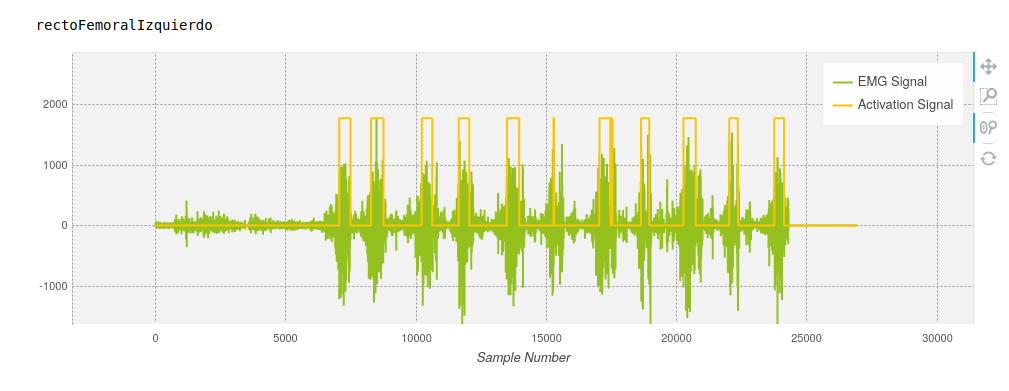
\includegraphics[width=1.0\textwidth]{imagenes/s3 serie 2 dia 2.png}
    \caption{ s3 serie 2 día 2: ejemplo de activación muscular}
    \label{fig:s1 serie 1 dia 1 error}
    \end{figure}
    
    Como se puede apreciar, en este archivo de EMG, solo había registradas 11 repeticiones, por lo que no es válido para nuestro estudio.



\section{Procesamiento de datos: diferentes modelos de estudio \label{anexo modelos}}

    \subsubsection{Canal 1, canal 2, canal 3, canal 4}
    Los archivos de entrenamiento-testeo obtenidos de cada canal tienen el mismo formato, solo cambia el valor de de las características obtenidas. Debido a ello solo se muestra el archivo del canal 1.
        \begin{figure}[!ht]
            \centering
            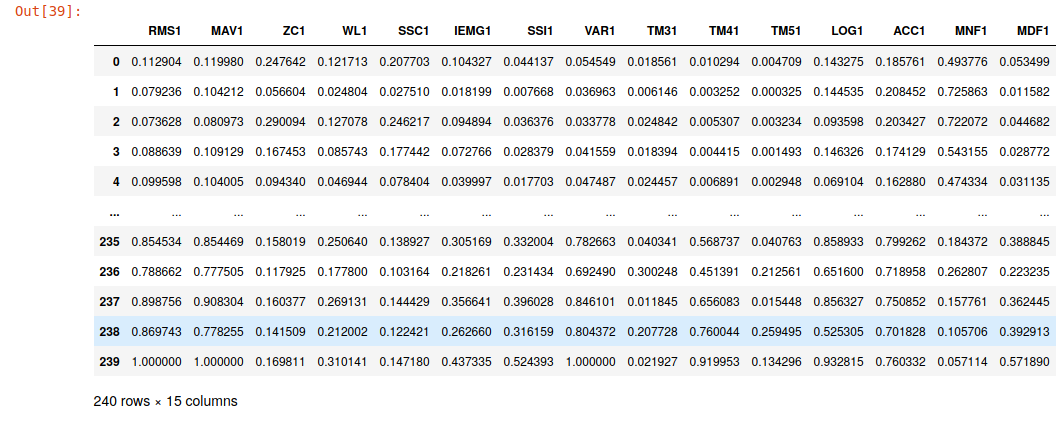
\includegraphics[width=1.0\textwidth]{imagenes/datos canal 1.png}
            \caption{Archivo entrenamiento-testeo del canal 1}
            \label{fig:archivo1}
        \end{figure}
   
   \newpage     
    \subsubsection{Canal 1,2}
        \begin{figure}[ht]
            \centering
            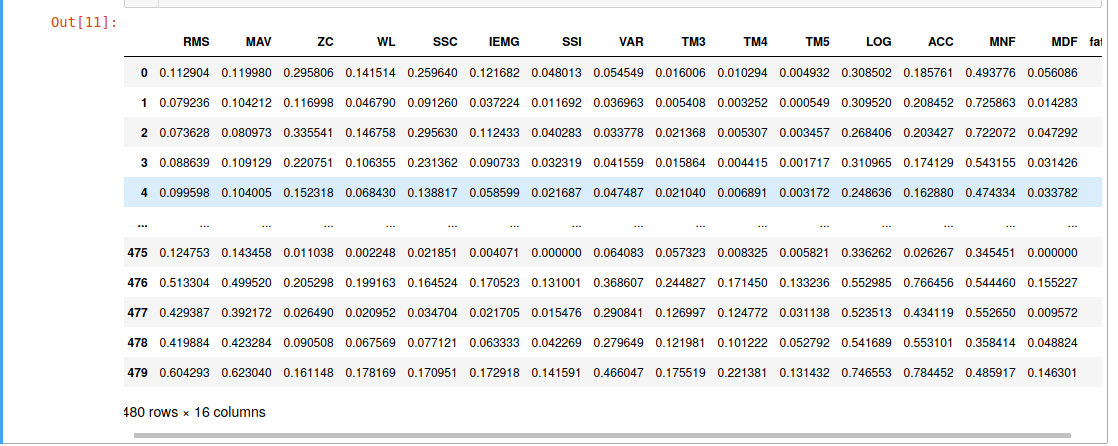
\includegraphics[width=1.0\textwidth]{imagenes/datos canal12.png}
            \caption{Archivo entrenamiento-testeo del canal 1,2}
            \label{fig:archivo12}
        \end{figure}
        
      
    \subsubsection{Canal 3,4}
        \begin{figure}[ht]
            \centering
            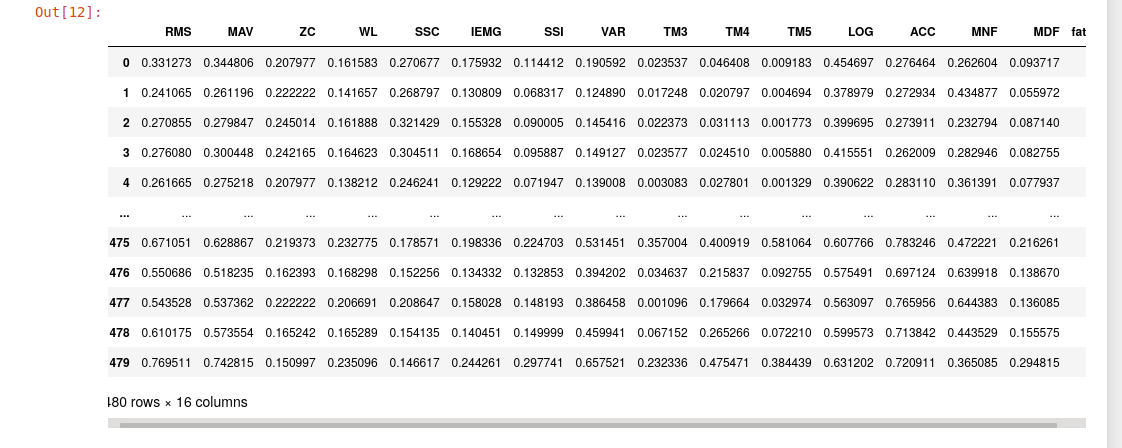
\includegraphics[width=1.0\textwidth]{imagenes/datos canal 34.png}
            \caption{Archivo entrenamiento-testeo del canal 3,4}
            \label{fig:archivo34}
        \end{figure}
        
        
        \newpage
    \subsubsection{Canal Total}
        \begin{figure}[ht]
            \centering
            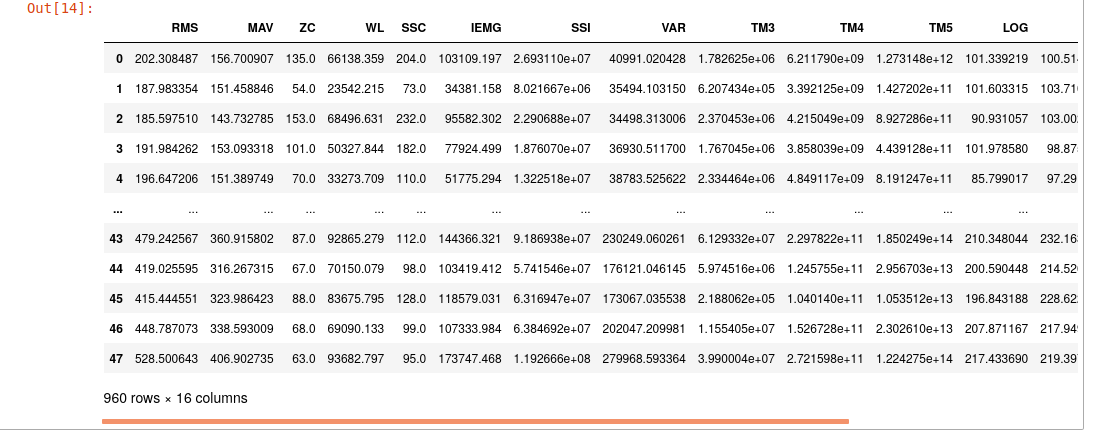
\includegraphics[width=1.0\textwidth]{imagenes/datos canal total.png}
            \caption{Archivo entrenamiento-testeo del canal total}
            \label{fig:archivototal}
        \end{figure}


\section{Selección de características: RFE \label{anexo rfe}}
	
	Tabla donde se muestran las características escogidas por el algoritmo RFE para el diseño de los clasificadores.
	\begin{table}[!ht]
    \centering
    \caption{Características seleccionadas para cada canal }
    
    \vspace{0.5cm}
    \scalebox{0.8}{
            \begin{tabular}{lllll}
                
                          &            N = 1 &       N = 2 &       N = 5 \\
                
                {\textbf{canal 1}} &    IEMG &  WL, IEMG &    ZC, WL, IEMG, TM4, ACC \\ \hline
                         
                
                {\textbf{canal 2}} &   IEMG &   IEMG, MDF&    ZC, WL, IEMG, VAR, MDF\\\hline
                          
                
                {\textbf{canal 3}} &    RMS  &  RMS, TM4 &   RMS, ZC, TM4, LOG, ACC\\\hline
                         
                
                {\textbf{canal 4}} &    MDF&   SSI, MDF&   ZC, SSI, TM3, TM4, MDF\\\hline
                          
                
                {\textbf{canal total}} & IEMG   & IEMG, SSI  & RMS, WL, SSC, IEMG, SSI  \\\hline
                         
                
                {\textbf{canal 1,2}} &   RMS   & RMS, VAR   &   RMS, IEMG, VAR, TM4, TM5   \\\hline
                         
                
                {\textbf{canal 3,4}} &    RMS  & RMS, VAR    &  RMS, MAV, SSI, VAR, MDF    \\
                          
                
            \end{tabular}   
    }
    
    \end{table}

\newpage


\section{Extracción de características  }

    \subsection{Implementación \label{anexocaracImple}}
A continuación el listado de todas las características implementadas junto con el código fuente correspondiente.

Con respecto a las características del dominio del tiempo:

\begin{itemize}
\item Root mean square (RMS)
\begin{lstlisting}[language=Python]
def RMS(datos,ratio):
    
    datosDevueltos=np.array([])
   
    if (ratio==0):
        return None

    i=0
    while i < datos.size:
        
        ratioN=0
        j=i
        i=i+int(ratio)
        sumaLocal=0
        #Para cada i , recorro sus "ratio" siguientes
        while j < i and j < datos.size:
            sumaLocal=sumaLocal+(datos[j]*datos[j])
            j=j+1
            ratioN=ratioN+1
         
        
        sumaTotal=sumaLocal/ratioN
        resultado=math.sqrt(sumaTotal) 
        
        datosDevueltos=np.append(datosDevueltos,resultado)
            
    
    

    return range(datosDevueltos.size),datosDevueltos
\end{lstlisting}

\newpage
\item Mean absolute value (MAV)
\begin{lstlisting}[language=Python]
def MAV(datos,ratio):
    
    
    datosDevueltos = np.array([])
    
    i=0
    while i < datos.size:
        
        ratioN=0
        j=i
        i=i+int(ratio)
        sumaLocal=0
        #Para cada i , recorro sus "ratio" siguientes
        while j < i and j < datos.size:
            sumaLocal=sumaLocal+abs(datos[j])
            j=j+1
            ratioN=ratioN+1
         
        
        datosDevueltos=np.append(datosDevueltos,sumaLocal/ratioN)
        
    return range(datosDevueltos.size),datosDevueltos
\end{lstlisting}

\item Zero crossing (ZC) con umbral de 0,01
\begin{lstlisting}[language=Python]
def ZC(datos,ratio,voltajeUmbral=0.01):
    
    
    datosDevueltos=np.array([])
    i=0
    while i < datos.size:
 
        j=i
        contadorLocal=0
        i+=int(ratio)
        
        while j < i-1 and j< datos.size-1:
        
            if (((datos[j] > 0 and datos[j+1]<0) or (datos[j]<0 and datos[j+1]>0)) and (abs(datos[j]-datos[j+1])>= voltajeUmbral)):
                contadorLocal+=1
                
            j+=1
        
        
        #if (contadorLocal != 0):
        datosDevueltos=np.append(datosDevueltos,contadorLocal)
          
        
        
    return range(datosDevueltos.size),datosDevueltos
\end{lstlisting}

\newpage
\item Waveform length (WL)
\begin{lstlisting}[language=Python]
def WL(datos,ratio):
    
    datosDevueltos=np.array([])
    i=0
    
    while i < datos.size:
        
        j=i
        sumaLocal=0
        i+=int(ratio)
        
        while j < i-1 and j< datos.size-1:
            sumaLocal=sumaLocal+abs(datos[j+1]-datos[j])
            j+=1
            
            
            
        datosDevueltos=np.append(datosDevueltos,sumaLocal)
    
    return range(datosDevueltos.size),datosDevueltos
\end{lstlisting}

\item Slope sign change (SSC) con umbral de 0,01
\begin{lstlisting}[language=Python]
def SSC(datos,ratio,voltajeUmbral=0.01):
    
    datosDevueltos=np.array([])
    #Dado que compara x(i) con x(i-1) y x(i+1)
    i=1
    while i < datos.size:
 
        j=i
        contadorLocal=0
        i+=int(ratio)
        #-2 dado que i comienza en 1
        while j < i-2 and j< datos.size-1:
            if(((datos[j]> datos[j-1] and datos[j]>datos[j+1]) or (datos[j] < datos[j-1] and datos[j]<datos[j+1] )) and (abs(datos[j]-datos[j+1])>= voltajeUmbral or abs(datos[j]-datos[j-1])>=voltajeUmbral)):
                contadorLocal+=1
                
            j+=1
        
        
        #if (contadorLocal != 0):
        datosDevueltos=np.append(datosDevueltos,contadorLocal)
          
        
        
    return range(datosDevueltos.size),datosDevueltos
\end{lstlisting}


\newpage
\item Integrated EMG (IEMG)
\begin{lstlisting}[language=Python]
def IEMG(datos,ratio):
    
    datosDevueltos = np.array([])
    
    i=0
    while i < datos.size:
        
        j=i
        i=i+int(ratio)
        sumaLocal=0
        #Para cada i , recorro sus "ratio" siguientes
        while j < i and j < datos.size:
            sumaLocal=sumaLocal+abs(datos[j])
            j=j+1
         
        
        datosDevueltos=np.append(datosDevueltos,sumaLocal)
        
    return range(datosDevueltos.size),datosDevueltos
\end{lstlisting}

\item Simple square integral (SSI)
\begin{lstlisting}[language=Python]
def SSI(datos,ratio):
    
    datosDevueltos = np.array([])
    
    i=0
    while i < datos.size:
        
        j=i
        i=i+int(ratio)
        sumaLocal=0
        #Para cada i , recorro sus "ratio" siguientes
        while j < i and j < datos.size:
            sumaLocal=sumaLocal+(datos[j]*datos[j])
            j=j+1
         
        
        datosDevueltos=np.append(datosDevueltos,sumaLocal)
        
    return range(datosDevueltos.size),datosDevueltos
\end{lstlisting}
\newpage
\item Variance of EMG (VAR)
\begin{lstlisting}[language=Python]
def VAR(datos,ratio):
    
    datosDevueltos=np.array([])
   
    i=0
    while i < datos.size:
        
        ratioN=0
        j=i
        i=i+int(ratio)
        sumaLocal=0
        #Para cada i , recorro sus "ratio" siguientes
        while j < i and j < datos.size:
            sumaLocal=sumaLocal+(datos[j]*datos[j])
            j=j+1
            ratioN=ratioN+1
         
        
        if (ratioN == 1):
            ratioN=2
            
        resultado=sumaLocal/(ratioN-1)
        
        datosDevueltos=np.append(datosDevueltos,resultado)
            
    
    

    return range(datosDevueltos.size),datosDevueltos
\end{lstlisting}

\item Absolute value 3rd (TM3)
\begin{lstlisting}[language=Python]
def TM3(datos, ratio):
    
    datosDevueltos=np.array([])
    
    
    i=0
    while i < datos.size:
        ratioN=0
        j=i
        i=i+int(ratio)
        sumaLocal=0
        while j< i and j< datos.size:
            sumaLocal=sumaLocal+pow(datos[j],3)
            j=j+1
            ratioN=ratioN+1
            
        resultado=abs(sumaLocal/ratioN)
        
        datosDevueltos=np.append(datosDevueltos,resultado)
        
    return range(datosDevueltos.size),datosDevueltos
\end{lstlisting}
\newpage
\item Absolute value 4th (TM4)
\begin{lstlisting}[language=Python]
def TM4(datos, ratio):
    
    datosDevueltos=np.array([])
    
    
    i=0
    while i < datos.size:
        ratioN=0
        j=i
        i=i+int(ratio)
        sumaLocal=0
        while j< i and j< datos.size:
            sumaLocal=sumaLocal+pow(datos[j],4)
            j=j+1
            ratioN=ratioN+1
            
        resultado=sumaLocal/ratioN
        
        datosDevueltos=np.append(datosDevueltos,resultado)
        
    return range(datosDevueltos.size),datosDevueltos
\end{lstlisting}

\item Absolute value 5th (TM5)
\begin{lstlisting}[language=Python]
def TM5(datos, ratio):
    
    datosDevueltos=np.array([])
    
    
    i=0
    while i < datos.size:
        ratioN=0
        j=i
        i=i+int(ratio)
        sumaLocal=0
        while j< i and j< datos.size:
            sumaLocal=sumaLocal+pow(datos[j],5)
            j=j+1
            ratioN=ratioN+1
            
        resultado=abs(sumaLocal/ratioN)
        
        datosDevueltos=np.append(datosDevueltos,resultado)
        
    return range(datosDevueltos.size),datosDevueltos
\end{lstlisting}


\newpage
\item Log detector (LOG)
\begin{lstlisting}[language=Python]
def LOG(datos,ratio):
    
    datosDevueltos=np.array([])
    
    i=0
    while i < datos.size:
        ratioN=0
        j=i
        i=i+int(ratio)
        sumaLocal=0
        while j< i and j< datos.size:
            if(datos[j] != 0):
                sumaLocal=sumaLocal+math.log(abs(datos[j]))
            j=j+1
            ratioN=ratioN+1
            
        resultado=math.exp(sumaLocal/ratioN)
        
        datosDevueltos=np.append(datosDevueltos,resultado)
        
    return range(datosDevueltos.size),datosDevueltos
\end{lstlisting}

\item Average amplitude change (ACC)
\begin{lstlisting}[language=Python]
def ACC(datos,ratio):
    
    datosDevueltos=np.array([])
    i=0
    
    while i < datos.size:
        
        j=i
        sumaLocal=0
        ratioN=1
        i+=int(ratio)
        
        while j < i-1 and j< datos.size-1:
            sumaLocal=sumaLocal+abs(datos[j+1]-datos[j])
            j+=1
            ratioN+=1
            
            
            
        datosDevueltos=np.append(datosDevueltos,sumaLocal/ratioN)
    
    return range(datosDevueltos.size),datosDevueltos
\end{lstlisting}
\end{itemize}

\newpage
Con respecto al dominio de la frecuencia :
\begin{itemize}
\item Median frecuency (MDF)
\begin{lstlisting}[language=Python]
def MDF(datos,ratio,fs=1024.0):
    
    datosDevueltos=np.array([])
    lista=[]
    datosProcesados=[]
   
    if (ratio==0):
        return None

    
    i=0
    while i< len(datos):
        
        lista.append(datos[i])
        if (len(lista)==ratio or i == len(datos)-1):
            frecuencia,poder = signal.welch(lista,fs,nperseg=len(lista))
            #Lista de vectores
            datosProcesados.append(poder)
            lista.clear()
        i=i+1
        
    
    for seccion in datosProcesados:
        suma=seccion.sum()/2
        datosDevueltos=np.append(datosDevueltos,suma)
    
    return range(datosDevueltos.size),datosDevueltos
\end{lstlisting}

\item Mean frecuency (MNF)
\begin{lstlisting}[language=Python]
def MNF(datos,ratio,fs=1024.0):
    
    datosDevueltos=np.array([])
    lista=[]
    datosPod=[]
    datosFre=[]
    
    if (ratio==0):
        return None

    
    i=0
    while i< len(datos):
        
        lista.append(datos[i])
        if (len(lista)==ratio or i == len(datos)-1):
            frecuencia,poder = signal.welch(lista,fs,nperseg=len(lista))
            datosPod.append(poder)
            datosFre.append(frecuencia)
            lista.clear()
        i=i+1
        
    
    suma=[]
    
    for i,j in zip(datosPod, datosFre):
        sumaNumerador=0
        sumaDenominador=0
        for datosP,datosF in zip(i,j):
            sumaNumerador=sumaNumerador+(datosP*datosF)
            sumaDenominador=sumaDenominador+datosP
            

        datosDevueltos=np.append(datosDevueltos,sumaNumerador/sumaDenominador)

    
    return range(datosDevueltos.size),datosDevueltos
\end{lstlisting}
\end{itemize}
    
    \subsection{Evaluación \label{anexo caracteristicas}}

Lista de gráficas de ejemplo para demostrar el funcionamiento de la extracción de características.
Se ha tomado la muestra del sujeto número 16, en la serie 3 del día 1. A continuación las gráficas relativas a cada una de las características implementadas:

\begin{figure}[ht]
	\centering
  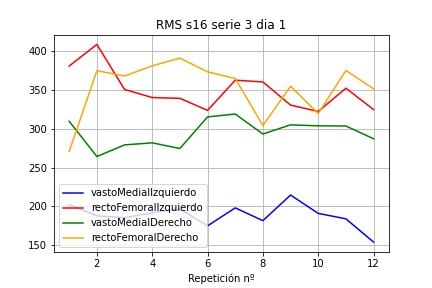
\includegraphics[width=1.0\textwidth]{imagenes/caracteristicas/RMS s16 serie 3 dia 1.jpg}
  \caption{ RMS}
  \label{fig:rms}
\end{figure}

\begin{figure}[ht]
	\centering
  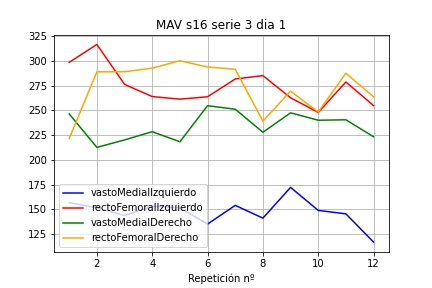
\includegraphics[width=1.0\textwidth]{imagenes/caracteristicas/MAV s16 serie 3 dia 1.jpg}
  \caption{MAV}
  \label{fig:mav}
\end{figure}

\begin{figure}[ht]
	\centering
  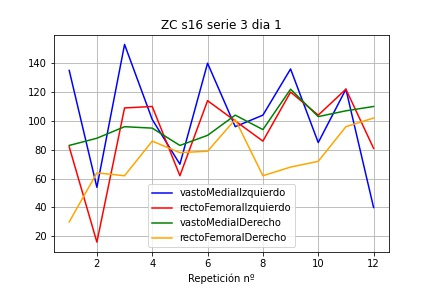
\includegraphics[width=1.0\textwidth]{imagenes/caracteristicas/ZC s16 serie 3 dia 1.jpg}
  \caption{ ZC con umbral de 0,01}
  \label{fig:zc}
\end{figure}


\begin{figure}[ht]
	\centering
  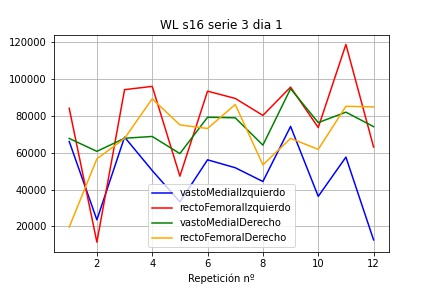
\includegraphics[width=1.0\textwidth]{imagenes/caracteristicas/WL s16 serie 3 dia 1.jpg}
  \caption{ WL}
  \label{fig:wl}
\end{figure}



\begin{figure}[ht]
	\centering
  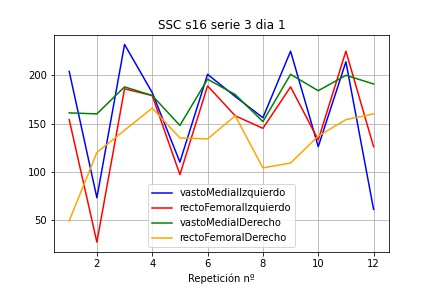
\includegraphics[width=1.0\textwidth]{imagenes/caracteristicas/SSC s16 serie 3 dia 1.jpg}
  \caption{ SSC con umbral de 0,01}
  \label{fig:ssc}
\end{figure}


\begin{figure}[ht]
	\centering
  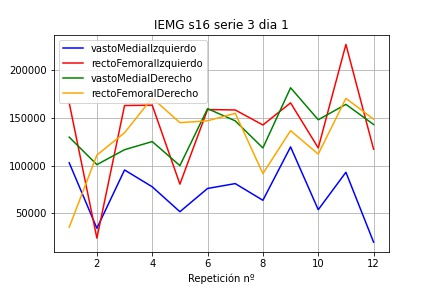
\includegraphics[width=1.0\textwidth]{imagenes/caracteristicas/IEMG s16 serie 3 dia 1.jpg}
  \caption{ IEMG}
  \label{fig:iemg}
\end{figure}

\begin{figure}[ht]
	\centering
  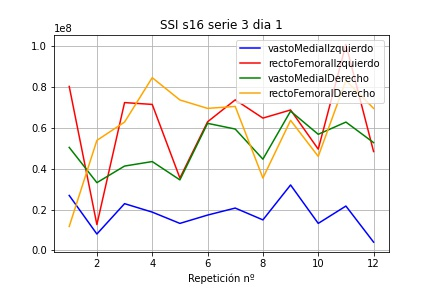
\includegraphics[width=1.0\textwidth]{imagenes/caracteristicas/SSI s16 serie 3 dia 1.jpg}
  \caption{ SSI}
  \label{fig:ssi}
\end{figure}
\begin{figure}[ht]
	\centering
  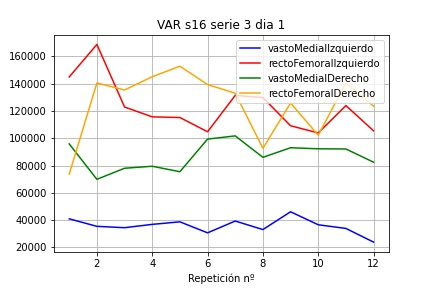
\includegraphics[width=1.0\textwidth]{imagenes/caracteristicas/VAR s16 serie 3 dia 1.jpg}
  \caption{ VAR}
  \label{fig:var}
\end{figure}
\begin{figure}[ht]
	\centering
  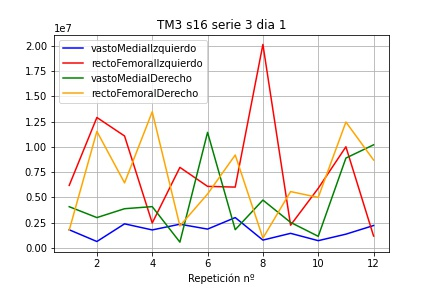
\includegraphics[width=1.0\textwidth]{imagenes/caracteristicas/TM3 s16 serie 3 dia 1.jpg}
  \caption{ TM3}
  \label{fig:TM3}
\end{figure}

\begin{figure}[ht]
	\centering
  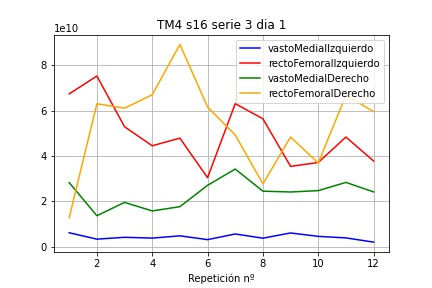
\includegraphics[width=1.0\textwidth]{imagenes/caracteristicas/TM4 s16 serie 3 dia 1.jpg}
  \caption{ TM4}
  \label{fig:tm4}
\end{figure}
\begin{figure}[ht]
	\centering
  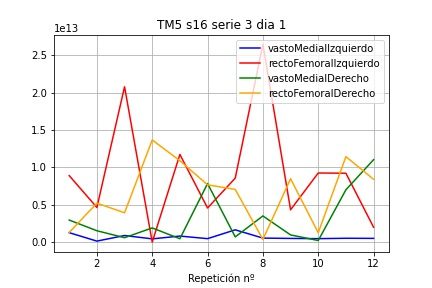
\includegraphics[width=1.0\textwidth]{imagenes/caracteristicas/TM5 s16 serie 3 dia 1.jpg}
  \caption{ TM5}
  \label{fig:tm5}
\end{figure}

\begin{figure}[ht]
	\centering
  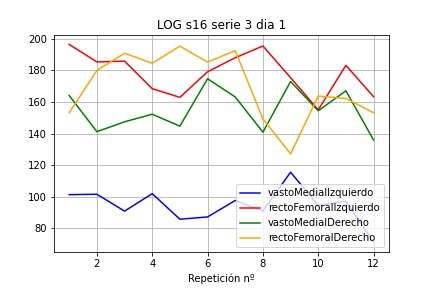
\includegraphics[width=1.0\textwidth]{imagenes/caracteristicas/LOG s16 serie 3 dia 1.jpg}
  \caption{ LOG}
  \label{fig:log}
\end{figure}

\begin{figure}[ht]
	\centering
  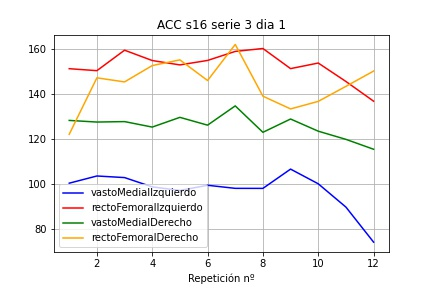
\includegraphics[width=1.0\textwidth]{imagenes/caracteristicas/ACC s16 serie 3 dia 1.jpg}
  \caption{ ACC}
  \label{fig:acc}
\end{figure}
\begin{figure}[ht]
	\centering
  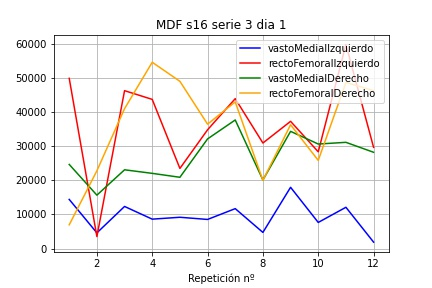
\includegraphics[width=1.0\textwidth]{imagenes/caracteristicas/MDF s16 serie 3 dia 1.jpg}
  \caption{ MDF}
  \label{fig:mdf}
\end{figure}
\begin{figure}[ht]
	\centering
  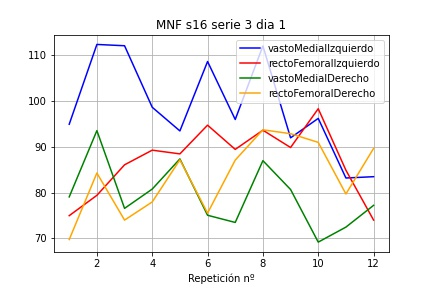
\includegraphics[width=1.0\textwidth]{imagenes/caracteristicas/MNF s16 serie 3 dia 1.jpg}
  \caption{ MNF}
  \label{fig:mnf}
\end{figure}
